\documentclass[12pt, openany]{report}
\usepackage[utf8]{inputenc}
\usepackage[T1]{fontenc}
\usepackage{amsmath,amsfonts,amssymb}
\usepackage{multicol}
\usepackage[a4paper,left=2.5cm,right=2.5cm,top=2.5cm,bottom=2.5cm]{geometry}
\usepackage[english]{babel}
\usepackage{libertine}
\usepackage{gensymb}
\usepackage{tabularray}
\usepackage{nicefrac}
\usepackage{graphicx}
\usepackage{steinmetz}
\usepackage{wrapfig}
\usepackage{float}
\usepackage{algorithm}
\usepackage{algpseudocode}
\usepackage[skins,many]{tcolorbox}
\usepackage{enumitem}
\usepackage{pythonhighlight}
\usepackage{empheq}
\usepackage{mathpazo}
\usepackage{xfrac}
\usepackage{textcomp}
%\usepackage[]{titletoc}
\usepackage{nicematrix}
\usepackage{titlesec}
\usepackage{mathtools}
\usepackage{caption}
\usepackage{subcaption}
\usepackage[bottom]{footmisc}
\usepackage{pdfpages}
\usepackage{tabularx}
\usepackage{amsthm}
\titleformat{\chapter}[display]
  {\normalfont\bfseries}{}{0pt}{\Huge}
\usepackage{hyperref}
\newcommand{\hsp}{\hspace{20pt}}
\newcommand{\HRule}{\rule{\linewidth}{0.5mm}}
\newcommand{\R}{\mathbb{R}}
\newcommand\independent{\protect\mathpalette{\protect\independenT}{\perp}}
\def\independenT#1#2{\mathrel{\rlap{$#1#2$}\mkern2mu{#1#2}}}

\usepackage{apptools}
    \titleformat{\chapter}[hang]{\bfseries\huge}{\IfAppendix{\appendixname~}{\relax}\thechapter\IfAppendix{.}{.}}{\IfAppendix{0.333em}{2pc}}{}

\titlespacing {\chapter}{0pt}{0pt}{40pt}

\usepackage[nottoc]{tocbibind}
\usepackage{keyval}
\usepackage{kvoptions}
\usepackage{fancyvrb}
\usepackage{ifthen}
\usepackage{calc}
\usepackage{pdftexcmds}
\usepackage{etoolbox}
\usepackage{xstring}
\usepackage{xcolor}
\usepackage{lineno}
\usepackage{tikz}
\usepackage{circuitikz}
\usetikzlibrary{patterns,arrows,decorations.pathreplacing,babel}

\usepackage[]{minted}
\newminted{python}{
    linenos=true,
    bgcolor=lightgray,
    tabsize=4,
    gobble=8,
    fontfamily=courier,
    fontsize=\small,
    xleftmargin=5pt,
    xrightmargin=5pt
}

\titleformat{\chapter}[display]
  {\normalfont\bfseries}{}{0pt}{\Huge}

% Define a new tcolorbox style with a red border and transparent interior
\tcbset{
    redbox/.style={
        enhanced,
        colframe=red,
        colback=white,
        boxrule=1pt,
        sharp corners,
        before skip=10pt,
        after skip=10pt,
        box align=center,
        width=\linewidth-2pt, % Adjust the width dynamically
    }
}
\newcommand{\boxedeq}[1]{
\begin{tcolorbox}[redbox]
    \begin{align}
        #1
    \end{align}
\end{tcolorbox}
}
\usepackage[]{titletoc}
\titleformat{\chapter}[display]
  {\normalfont\bfseries}{}{0pt}{\Huge}
\def\independenT#1#2{\mathrel{\rlap{$#1#2$}\mkern2mu{#1#2}}}

\theoremstyle{definition}
\newtheorem{thm}{Theorem}[chapter]
\newtheorem{definition}[thm]{Definition}
\newtheorem{exmp}[thm]{Example} 
\newtheorem{lem}[thm]{Lemma}
\newtheorem{prop}[thm]{Property}
\newtheorem{crl}[thm]{Corollary}

\usepackage{apptools}
    \titleformat{\chapter}[hang]{\bfseries\huge}{\IfAppendix{\appendixname~}{\relax}\thechapter\IfAppendix{.}{.}}{\IfAppendix{0.333em}{2pc}}{}

\titlespacing {\chapter}{0pt}{0pt}{40pt}


\begin{document}


\begin{titlepage}
    \begin{sffamily}
    \begin{center}
        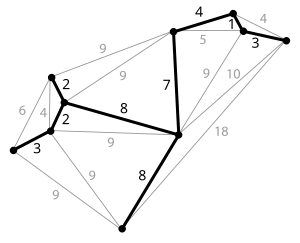
\includegraphics[scale=0.75]{img/page_de_garde.png} \\[1cm]
        \HRule \\[0.4cm]
        { \huge \bfseries LINMA2450 Combinatorial Optimization \\[0.4cm] }
    
        \HRule \\[1.5cm]
        \textsc{\LARGE Simon Desmidt}\\[1cm]
        \vfill
        \vspace{2cm}
        {\large Academic year 2024-2025 - Q1}
        \vspace{0.4cm}
         
        
\includegraphics[width=0.15\textwidth]{img/epl.png}
        
        UCLouvain\\
    
    \end{center}
    \end{sffamily}
\end{titlepage}

\setcounter{tocdepth}{1}
\tableofcontents
\chapter{Introduction}
\section{Continuous vs Combinatorial optimization}
A continuous optimization problem is expressed as 
\begin{equation}\label{eq:1}
    \max/\min f(x)
\end{equation} 
such that \(x\in \Omega\), where \(f:\mathbb{R}^n \rightarrow \mathbb{R}\) and \(\Omega \subseteq \mathbb{R}^n\), where \(\Omega\) does not have isolated points. \\
A combinatorial optimization problem has the additional constraint that \[x\in \Omega \cap \mathbb{Z}^n\] which can be a finite set of values. If finite, it is not solvable by exhaustive search, as it can contain loads of points even for small scale problems.
\section{Upper/Lower bound}
Let \(f^*=\max \{f(x):\quad x\in \Omega\cap \mathbb{Z}^n\}\) be the optimal value for a given problem.
\begin{itemize}
    \item Any lower bound for \(f^*\) is called primal bound. One way to get primal bounds is to find feasible points, because if \(x\in \Omega\cap \mathbb{Z}^n\), then \(f_L = f(x)\le f^*\).
    \item Any upper bound for \(f^*\) is called dual bound. One way to get this upper bound is to use relaxation : \[f^* \le \max_x \{f(x):\quad x\in \Omega\} = f_{\mathcal{U}}\] Thus if \(f_{\mathcal{U}}-f(x)\le \varepsilon\), we have a certificate that \(x\) is an \(\varepsilon\)-approximate solution of \ref{eq:1}.
\end{itemize}
\chapter{Knapsak problem}
Suppose that we have the following : 
\begin{itemize}
    \item a bag;
    \item a set of objects that we want to put in the bag;
    \item each object has a value.
\end{itemize}
The objective of this problem is to select the objects to put in the bag in order to maximze the total value of the objects in the bag, such that the objects fit in the bag. We can only put nonnegative integer amounts of each object in the bag. 
\subsection{Mathematical formulation}
\begin{itemize}
    \item \(b\) : the volume of the bag
    \item \(n\) : the number of types of objects
    \item \(0<a_j\le b\) : the volume of one unit of object \(j\)
    \item \(c_j>0\) : the value of one unit of object \(j\)
    \item \(x_j\) : the amount of object \(j\) that is put in the bag (VARIABLES)
\end{itemize}
The Linear Integer Programming Problem expression here is 
\begin{equation}\label{eq:2}
    \max \sum_{j=1}^n x_jc_j \quad \text{such that}\quad \begin{cases}
        a^Tx \le b\\
        x_j\in \mathbb{N} \quad \forall j=1,\dots,n
    \end{cases}
\end{equation}
Let us now suppose that 
\begin{equation}\label{eq:3}
    \frac{c_1}{a_1}\ge \frac{c_2}{a_2} \ge \dots \ge \frac{c_n}{a_n}
\end{equation}
The greedy approach is to put in the bag the maximum amount possible of object 1, then 2, and so on. The amount of object \(j\) in the bag will therefore be 
\begin{equation}\label{eq:4}
    x_j^{(g)} = \left\lfloor \frac{b-\sum_{i=1}^{j-1} a_ix_i^{(g)}}{a_j} \right\rfloor \quad \forall j=1,\dots,n
\end{equation}
and the feasible point is \(x^{(g)}\) such that it \(j\) component is \(x_j^{(g)}\) calculated above. 
\begin{tcolorbox}[breakable,
                  colback=white,
                  colframe=white!75!black,
                  title={Theorem}]
    Let \(x^{(g)}\) be the feasible point to problem \ref{eq:2} given by the equation \ref{eq:4}, and suppose that the assumption \ref{eq:3} is true. Then,\[f\left(x^{(g)}\right) \ge \sfrac{1}{2} f^*\] that is, the Greedy Heuristics to a Knapsak problem gives a feasible point with a function value equal to at least 50\% of the optimal value.
\end{tcolorbox}
\chapter{Relaxation}
We will here study problems such that the relaxation of the integer constraint still gives the same solution, i.e. solving the discrete or continuous problem is equivalent.\\
\section{Linear problems}
\subsection{Definitions}
\begin{itemize}
    \item A matrix \(B\in \mathbb{Z}^{k\times k}\) is unimodular when it is invertible and \(B^{-1}\in \mathbb{Z}^{k\times k}\). 
    \item \(B\in \mathbb{Z}^{k\times k}\) is unimodular iff \(\det B\in \{-1,1\}\). 
    \item \(A\in \mathbb{Z}^{m\times n}\) is totally unimodular (TU) when every invertible submatrix of \(A\) is unimodular. 
    \item Let \(A\in \mathbb{Z}^{m\times n}\). If \(\det(B) \in \{-1,0,1\}\) for every square submatrix of \(A\), then A is TU.
\end{itemize}
\section{Resolution}\label{sec:main_th}
A linear problem of optimization can be written under the following general form :
\begin{equation}
    \max f(x) = c^Tx \qquad \text{ such that } Ax\le b
\end{equation}
We can use the simplex method in that problem, stating that the solution is one of the vertices of the feasible set (a polygon here). It is possible to rearrange the rows of \(A\) and \(b\) in such a way that we get
\begin{equation}
    \begin{pNiceArray}{c}
  B\\
  \hline
  C\\
\end{pNiceArray} \qquad \begin{pNiceArray}{c}
  b_{(1)} \\
  \hline
  b_{(2)}\\
\end{pNiceArray}
\end{equation}
With that, the solution \(x^* = \begin{pmatrix}
x^*_{(1)}\\ x^*_{(2)}\\ \end{pmatrix}
\) verifies 
\begin{equation}
    \begin{cases}
        Bx_{(1)}^* = b_{(1)}\\
        x_{(2)}^* = 0\\
    \end{cases}
\end{equation}
B being non singular.
\begin{tcolorbox}[breakable,
                  colback=white,
                  colframe=white!75!black,
                  title={Theorem}]
    Let \(A\in \mathbb{Z}^{m\times n}\) be a matrix such that
    \begin{enumerate}
        \item \(A_{ij} \in \{-1,0,1\}\);
        \item Every column of \(A\) has at most 2 nonzero entries:
        \item There exists a partition\footnote{\(I_1\cap I_2 = \emptyset\) and \(I_1 \cup I_2 = \) the set.} \(I_1\cup I_2 = \{1,\dots,m\}\) such that, if the \(j\)th column of \(A\) has exactly 2 nonzero entries, then \(\sum_{i\in I_1} A_{ij} = \sum_{i\in I_2} A_{ij}\);
    \end{enumerate}
    Then \(A\) is TU.
\end{tcolorbox}
\chapter{Applications}
\section{Maximum Matching Problem}
\subsection{Definitions}
\begin{itemize}
    \item Given a graph \(G=(V,E)\), a matching of \(G\) is a subset of edges \(E'\subset E\) such that for every vertex \(v\in V\), there exists at most one edge \(e\in E'\) that is incident to it.
    \item Assume that \(V=\{v_1,\dots,v_m\}\) and \(E=\{e_1,\dots, e_n\}\). Given \(E'\subset E\), we can then associate it to the vector \(x'\in \{0,1\}\subset \mathbb{Z}^n\subset \mathbb{R}^n\) given by 
    \begin{equation}
        x_j' = \begin{cases}
            1 \text{ if } e_j \in E'\\
            0\text{ otherwise}
        \end{cases}
    \end{equation}
    \item Then, with this notation, we have 
    \begin{equation}
        |E'| = \mathbb{1}^Tx'
    \end{equation}
    \item Let us define the vertex-edge incidence matrix of \(G=(V,E)\) as the matrix \(M\in \mathbb{Z}^{m\times n}\) given by
    \begin{equation}
        M_{ij} = \begin{cases} 1 \text{ if }e_j\text{ is incident to }v_j\\ 0 \text{ otherwise}\\ \end{cases} \qquad i=1,\dots,m\qquad j=1,\dots,n
    \end{equation}
\end{itemize}
\subsection{Unweighted Problem}
The maximum unweighted matching problem is to find a subgraph of a bipartite graph for which the maximum number of nodes are related to max one other node. It can be expressed in an combinatorial optimization manner such as:
\begin{equation}
    \max \mathbb{1}^Tx \qquad \text{ such that } Mx\le \mathbb{1}_m \qquad x\in \{0,1\}^n
\end{equation}
We want to be able to use the theorem of section \ref{sec:main_th}. 
\begin{tcolorbox}[breakable,
    colback=white,
    colframe=white!75!black,
    title={Theorem}]
If \(G=(V,E)\) with \(|V| = m\) and \(|E|=n\) is a bipartite graph with no self-loop\footnote{Edge from a node to itself.}, then its vertex-edge incidence matrix \(M\in \mathbb{Z}^{m\times n}\) is a TU matrix.
\end{tcolorbox}
\subsection{Weighted Problem}
Let \(w_j\) be the weight associated to the edge \(e\in E\). The function to optimize then is \(w^Tx\), and the problem becomes 
\begin{equation}
    \max_{x\in \R^n} w^Tx \text{   such that   }Mx\le \mathbb{1}_m \qquad x\in \{0,1\}^n
\end{equation}
\section{Minimum Vertex Cover Problem}
\begin{definition}
    Given a graph \(G=(V,E)\), a vertex cover of \(G\) is a subset \(V'\subset V\) such that for every edge \(e=\{u,v\}\in E\), we have \(u\in V'\) or \(v\in V'\).
\end{definition}
The minimum vertex cover problem consists in minimizing the cardinality of \(V'\subset V\) such that \(V'\) is a vertex cover of \(G\). We define the vector \(u\in \R^m\) such that
\begin{equation}
    u_i = \begin{cases}
        1 \text{ if } v_i\in V'\\
        0\text{ otherwise}
    \end{cases}\qquad i=1,\dots,m
\end{equation}
The algebraic formulation of the problem is the following:
\begin{equation}\label{eq:mvcp_d}
    \min_{u\in \R^m}\mathbb{1}^Tu \text{ such that }M^Tu\ge \mathbb{1}_n\qquad u\in \{0,1\}^m
\end{equation}
If the graph is bipartite, then the incidence matrix \(M\) is TU, and the problem \eqref{eq:mvcp_d} is equivalent its relaxation:
\begin{equation}
    \min_{u\in \R^m}\mathbb{1}^Tu \text{ such that }M^Tu\ge \mathbb{1}_n\qquad u\in [0,1]^m
\end{equation}
Given a solution \(u^*\) of that problem, the desired vertex cover \(V^*\) will be the set \(V^* = \{v_i:u_i^*=1\}\). 
\section{Shortest Path Problem}
\begin{definition}
    A directed graph is a pair \(G=(V,A)\) where \(V\neq \emptyset\) is the set of vertices and \(A\subset V\times V\) is the set of arrows. If \((u,v)\in A\), the edge leaves \(u\) and arrives at \(v\).
\end{definition}
Let \(G=(V,A)\) be a directed graph with \(V=\{v_1,\dots,v_m\}\) and \(A=\{a_1,\dots,a_n\}\). Then, the vertex-arrow incidence matrix \(M^d\in \R^{m\times n}\) is defined such that 
\begin{equation}
    M_{ij}^d = \begin{cases}
        -1 \text{ if }a_j \text{ leaves }v_i\\
        1 \text{ if }a_j \text{ arrives at }v_i\\
        0 \text{ otherwise}
    \end{cases}
\end{equation}
\begin{definition}
    A path on \(G=(V,A)\) from vertex \(s\) to vertex \(t\) is a set of arrows \(P\subset A\) such that 
    \begin{equation}
        P=\{(\tilde v_1,\tilde v_2), (\tilde v_2,\tilde v_3), \dots, (\tilde v_{N-1},\tilde v_N)\}
    \end{equation}
    where \(\tilde v_1= s\), \(\tilde v_N=t\) and \(\tilde v_i\neq \tilde v_\ell\) if \(i\neq \ell\)\footnote{i.e. there is no cycle.}.
\end{definition}
Given a path \(P\subset A\), we can associate it to a vector \(x\in \R^n\) such that 
\begin{equation}
    x_j=\begin{cases}
        1\text{ if }a_j\in P\\
        0\text{ otherwise}
    \end{cases}
\end{equation}
Let \(c_j\) be the cost associated to arrow \(a_j\). Then, the shortest path problem can be formulated as 
\begin{equation}\label{eq:spp}
    \min_{x\in \R^n}c^Tx \text{   such that   }M^dx=b\qquad x\in \{0,1\}^n
\end{equation}
where \(b\) is a vector such that its first component is -1, its last is 1, and all others are zero. The condition \(M^dx=b\) translates the fact that all arrows of the path must be next to each other, and that the path starts in \(s\) and ends in \(t\). 
\begin{tcolorbox}[breakable,
    colback=white,
    colframe=white!75!black,
    title={Theorem}]
    Let \(G=(V,A)\) be a directed graph with \(|V|=m\) and \(|A|=n\). Denote by \(M^d\in\R^{m\times n}\) the vertex-arrow incidence matrix. If the graph has no self-loop, then \(M^d\) is TU.
\end{tcolorbox}
This means that once again, the combinatorial problem \eqref{eq:spp} is equivalent to its continuous relaxation. 
\begin{prop}
    If a matrix \(A\) is TU, then the matrices \(B=\begin{bmatrix}
        A \\
        I \\
    \end{bmatrix}\) and \(C=\begin{bmatrix}
        A\\ -A\\
    \end{bmatrix}\) are both also TU. This means that the condition \(x\in [0,1]^n\) can always be added to the TU incidence matrix and stay TU.
\end{prop}
\section{Maximum Flow Problem}
In this problem, we want to maximize the flow that we can send from node \(s\) to node \(t\), respecting the conservative law, i.e. at intermediate vertices, the flow that arrives is equal to the flow that leaves. \\
Let us define the matrix \(\Tilde M\) defined by the following:
\begin{equation}
    \Tilde M_{ij} = \begin{cases}
        1 & \text{ if } j\in \delta^{(+)}(i)\\
        -1 & \text{ if } j\in \delta^{(-)}(i)\\
        0 & \text{ otherwise}\\
    \end{cases} \forall i\in \{2,\dots,m-1\},j\in \{1,\dots, n\}
\end{equation}
where 
\begin{equation}
    \begin{cases}
        \delta^{(-)}(i) = \{j\in \{1,\dots,n\}:a_j\text{ leaves }v_i\}\\
        \delta^{(+)}(i) = \{j\in \{1,\dots,n\}:a_j\text{ arrives at }v_i\}
    \end{cases}
\end{equation}
In matrix form, the problem is
\begin{equation}
    \max_{x\in \R^n} \sum_{j\in \delta^{(-)}(i)}x_j \text{   such that   } \Tilde M=0\qquad 0\le x_j\le c_j \: \forall j=1,\dots,n
\end{equation}
The constraint containing \(\Tilde M\) is the conservation law. 
\section{Assignment Problem}
Suppose that we have $n$ tasks and $m$ agents. Every task should be done by some agent, and every agent is responsible for one and only one task. Let $h_{ij}$ be the "happiness" that agent $i$ will feel by doing task $j$. We want to maximize the total happiness of the agents. \\
Let $\R^{n\times n}$ be the decision variable such that 
\begin{equation}
    x_{ij} = \begin{cases}
        1& \text{ if the }j\text{th task is done by agent }i\\
        0& \text{ otherwise}
    \end{cases}
\end{equation}
Then the problem is formulated as 
\begin{equation}
    \max_{x\in \R^{n\times n}} \sum_{j=1}^{n}\sum_{i=1}^n h_{ij}x_{ij}\text{   such that   }\begin{cases}
        \sum_{j=1}^n x_{ij} = 1\qquad i=1, \dots, n\\
        \sum_{j=1}^n x_{ij} = 1\qquad j=1, \dots, n\\
    \end{cases}
\end{equation}
Let us put all this in matrix form, defining the vector $x_{n^2}$ and the matrix $A_{2n\times n^2}$ such that, for \(n=2\), we have
\begin{equation}
    \begin{pmatrix}
        1 & 1 & 0 & 0 \\
        0 & 0 & 1 & 1 \\
        1 & 0 & 1 & 0 \\
        0 & 1 & 0 & 1 \\
    \end{pmatrix}\begin{pmatrix}
        x_{11}\\ x_{21} \\ x_{12} \\ x_{22}\\
    \end{pmatrix} = \begin{pmatrix}
        1\\ 1\\ 1\\ 1\\
    \end{pmatrix}
\end{equation}
It is easy to show that the matrix $A$ is TU, and thus the problem is written in the general form:
\begin{equation}
    \max_{x\in \R^{n^2}} h^Tx \text{   such that   } Ax=\mathbb{1}_{2n}\qquad x\in \{0,1\}^{n^2}
\end{equation}
\section{Mininimum Cut Problem}
\begin{definition}
    Given a directed graph $G=(V,A)$ and $s,t\in V,s\neq t$, an $s-t$ cut is a pair $(S,T)$ such that $V=S\cup T$, $S\cap T=\emptyset$, $s\in S$ and $t\in T$.
\end{definition}
Suppose that $V=\{v_1,\dots,v_n\}$ with $s=v_1$ and $t=v_n$. Let $\Tilde A=\{(i,j)|(v_i,v_j)\in A\}$. We define $c_{ij}$ as the capacity of the arrow $(v_i,v_j)$, and finally $W\in \R^{n\times n}$ and $u\in \R^n$:
\begin{equation}
    W_{ij} = \begin{cases}
        1& \text{ if } v_i \in S\text{ and } v_j\in T\\
        0& \text{ otherwise}    
    \end{cases}
\end{equation}
\begin{equation}
    u_i = \begin{cases}
        1& \text{ if } v_i \in S\\
        0& \text{ otherwise}    
    \end{cases}
\end{equation}
The Minimum $s-t$ cut problem is the problem of finding an $s-t$ cut with minimum capacity:
\begin{equation}
    \min_{u,W} \sum_{(i,j)\in \Tilde A}c_{ij}W_{ij}\text{ such that } \begin{cases}
        W_{ij}\ge u_i-u_j & \forall (i,j)\in \Tilde A, i\neq 1, j \neq n\\
        W_{1j}\ge 1-u_j & \forall (1,j)\in \Tilde A\\
        W_{in}\ge u_i & \forall (i,n)\in \Tilde A\\
        W_{ij}\in \{0,1\}& \forall (i,j)\in \Tilde A\\
        u_i \in \{0,1\} & \forall i\in \{1,\dots,n\}\\
    \end{cases}
\end{equation}
\begin{thm}
    The Maximum $s-t$ Flow Problem and the Minimum $s-t$ Cut Problem are strongly dual to each other.
\end{thm}
\chapter{Submodularity}
\section{Submodular function}
\begin{definition}
    Given a finite set $E$, let $\mathcal{P}(E)$ be the set of all subsets of $E$. We say that a function $f:\mathcal{P}(E)\rightarrow \R$ is a submodular function when for all subsets $A\subset B\subset E$ and for all $x\in E\setminus B$, we have 
    \begin{equation}
        f(A\cup \{x\})-f(A) \ge f(B\cup \{x\})-f(B)
    \end{equation}
    $f$ is said to be monotone if $f(A)\le f(B)\: \forall A\subset B$.
\end{definition}
Given a monotone submodular function $f:\mathcal{P}(E)\rightarrow \R_+$ and an integer $k\ge 1$, consider the problem of maximizing $f$ subject to a cardinality constraint:
\begin{equation}\label{eq:cardinal}
    \max_{A\subset E} f(A) \text{ such that } |A| \le k
\end{equation}
\begin{algorithm}
    \caption{Greedy Method for Problem \eqref{eq:cardinal}}\label{algo:cardinal}
    \begin{algorithmic}[1]
    \State \textbf{Step 0:} Set $S_0=\emptyset$ and $i\coloneqq 0$.
    \State \textbf{Step 1:} If $i=k$, stop.
    \State \textbf{Step 2:} Set 
    \begin{equation}
        x_{i+1} = \arg\max_{x\in E\setminus S_i} f(S_i\cup \{x\})
    \end{equation}
    \State \textbf{Step 3:} Set $S_{i+1}=S_i\cup \{x_{i+1}\}$ and $i\coloneqq i+1$ and go back to Step 1.
    \end{algorithmic}
\end{algorithm}
\begin{tcolorbox}[breakable,
    colback=white,
    colframe=white!75!black,
    title={Theorem}]
Let $\{S_i\}_{i=0}^k$ be generated by Algorithm \ref{algo:cardinal}. If $S^*$ is a solution of \eqref{eq:cardinal}, then 
\begin{equation}
    f(S^*) -f(S_i) \le \left(1-\frac{1}{k}\right)^i f(S^*) \qquad \forall 0\le i \le k
\end{equation}
\end{tcolorbox}
This means that 
\begin{equation}
    f(S_k) \ge \left(1-\frac{1}{e}\right)f(S^*)\ge 0.63 f(S^*)
\end{equation}
\section{k-Medoids Problem}
Given a dataset $E\subset \R^n$ finite, find a subset $M\subset E$ with at most $k$ elements (called medoids) such that the sum of pairwise distances between medoids and elements of $E$ is minimized:
\begin{equation}
    \min_{M\subset E} L(M)\equiv \frac{1}{|E|}\sum_{v\in E} \min_{e\in M}\lVert e-v\rVert \text{    such that    } |M|\le k
\end{equation}
This is equivalent to 
\begin{equation}
    \max{M\subset E} f(M)\equiv L(\{e_0\})-L(M\cup \{e_0\})\text{    such that    } |M|\le k
\end{equation}
where $e_0$ is a phantom medoid. Practically, we have a dataset and find two medoids using Algorithm \ref{algo:cardinal}. With the above problem, we find the clusters of the dataset by assigning the points to the closest medoid. 
\end{document}